\chapter{Định thức}
\section{Định nghĩa và tính chất}
\subsection{Định nghĩa}
Cho $A$ là ma trận vuông cấp $n.$ Ta gọi ma trận $A\left( {\left. i \right|j} \right)$ là ma trận có được từ $A$ bằng cách \textit{xóa đi dòng $i$ và cột $j$} của $A.$ Rõ ràng ma trận $A\left( {\left. i \right|j} \right)$ có cấp là $n - 1.$\\
Cho $A = \left( {a_{ij}} \right) \in M_n \left( {\mathbb{R}} \right).$  \textit{Định thức} của ma trận $A,$ được ký hiệu là $\left| A \right|$ (hay $\det \left( A \right)$) là một số thực được xác định bằng quy nạp theo $n$ như sau:
\begin{itemize}
\item Nếu $n = 1,$ nghĩa là $A = \left( a \right),$ thì $\left| A \right| = a.$
\item Nếu $n = 2,$ nghĩa là $A = \left( {\begin{array}{*{20}{c}}
  a&b \\ 
  c&d 
\end{array}} \right),$ thì $\left| A \right| = ad - bc.$
\item Nếu $n > 2,$ nghĩa là
$A = \left( {\begin{array}{*{20}{c}}
  {{a_{11}}}&{{a_{12}}}&{...}&{{a_{1n}}} \\ 
  {{a_{21}}}&{{a_{22}}}&{...}&{{a_{2n}}} \\ 
  {...}&{...}&{...}&{...} \\ 
  {{a_{n1}}}&{{a_{n2}}}&{...}&{{a_{nn}}} 
\end{array}} \right),$ 
thì 
$$\left| A \right|\mathop  = \limits^{\text{dòng } 1} \sum\limits_{j = 1}^n {{a_{1j}}{{\left( { - 1} \right)}^{1 + j}}\left| {A\left( {\left. 1 \right|j} \right)} \right|} $$
$$ = {a_{11}}\left| {A\left( {\left. 1 \right|1} \right)} \right| - {a_{12}}\left| {A\left( {\left. 1 \right|2} \right)} \right| + ... + {a_{1n}}{\left( { - 1} \right)^{1 + n}}\left| {A\left( {\left. 1 \right|n} \right)} \right|.$$
\end{itemize}
\subsection{Quy tắc Sarrus $\left( {n = 3} \right)$}
Cho $A = \left( {\begin{array}{*{20}{c}}
  {{a_{11}}}&{{a_{12}}}&{{a_{13}}} \\ 
  {{a_{21}}}&{{a_{22}}}&{{a_{23}}} \\ 
  {{a_{31}}}&{{a_{32}}}&{{a_{33}}} 
\end{array}} \right).$ Theo định nghĩa của định thức, ta có
$$\left| A \right| = {a_{11}}\left| {\begin{array}{*{20}{c}}
  {{a_{22}}}&{{a_{23}}} \\ 
  {{a_{32}}}&{{a_{33}}} 
\end{array}} \right| - {a_{12}}\left| {\begin{array}{*{20}{c}}
  {{a_{21}}}&{{a_{23}}} \\ 
  {{a_{31}}}&{{a_{33}}} 
\end{array}} \right| + {a_{13}}\left| {\begin{array}{*{20}{c}}
  {{a_{21}}}&{{a_{22}}} \\ 
  {{a_{31}}}&{{a_{32}}} 
\end{array}} \right|$$
$$ = {a_{11}}{a_{22}}{a_{33}} + {a_{12}}{a_{23}}{a_{31}} + {a_{13}}{a_{21}}{a_{32}} - {a_{11}}{a_{23}}{a_{32}} - {a_{12}}{a_{21}}{a_{33}} - {a_{13}}{a_{22}}{a_{31}}.$$
Từ đây ta suy ra công thức Sarrus dựa vào sơ đồ sau
\begin{figure}[H]
\begin{center}
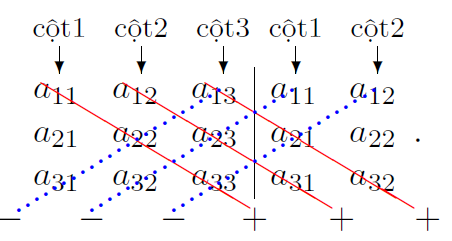
\includegraphics[scale=0.8]{C2_1}
\end{center}
\end{figure}
$$\left| A \right| = {a_{11}}{a_{22}}{a_{33}} + {a_{12}}{a_{23}}{a_{31}} + {a_{13}}{a_{21}}{a_{32}} - \left( {{a_{13}}{a_{22}}{a_{31}} + {a_{11}}{a_{23}}{a_{32}} + {a_{12}}{a_{21}}{a_{33}}} \right).$$
(Tổng ba đường chéo \textbf{đỏ} - tổng ba đường chéo \textbf{xanh})
\subsection{Khai triển định thức theo dòng và cột}
Cho $A = \left( {a_{ij}} \right) \in M_n \left( {\mathbb{R}} \right).$  Với mỗi $i,j \in \overline {1,n} ,$ ta gọi
$${c_{ij}} = {\left( { - 1} \right)^{i + j}}\left| {A\left( {\left. i \right|j} \right)} \right|$$
là \textit{phần bù đại số} của $a_{ij}.$
\begin{mybox}
\begin{theorem}
Cho $A = \left( {a_{ij}} \right) \in M_n \left( {\mathbb{R}} \right).$ Với mỗi $i,j \in \overline {1,n} ,$ ta gọi $c_{ij}$ là \textit{phần bù đại số} của $a_{ij}.$ Ta có công thức khai triển $\left| a \right|,$
\begin{itemize}
\item theo dòng $i:$ $\left| A \right| = \sum\limits_{k = 1}^n {{a_{ik}}{c_{ik}}} .$
\item theo dòng $j:$ $\left| A \right| = \sum\limits_{k = 1}^n {{a_{kj}}{c_{kj}}} .$
\end{itemize}
\end{theorem}
\end{mybox}
\begin{mybox}
\textbf{Nhận xét.} 
\[A\mathop  = \limits^{\text{ dòng }i} \sum\limits_{k = 1}^n {{a_{ik}}{{\left( { - 1} \right)}^{i + k}}\left| {A\left( {\left. i \right|k} \right)} \right|} \]
\[\begin{array}{*{20}{c}}
  {}&{\mathop  = \limits^{\text{cột } j} } 
\end{array}\sum\limits_{k = 1}^n {{a_{kj}}{{\left( { - 1} \right)}^{k + j}}\left| {A\left( {\left. k \right|j} \right)} \right|} \]
\end{mybox}
\begin{mybox}
\textbf{Lưu ý.} Khi tính định thức của ma trận ta nên chọn dòng hay cột có nhiều số $0$ để khai triển.
\end{mybox}
\begin{mybox}
\textbf{Mệnh đề.} Cho $A  \in M_n \left( {\mathbb{R}} \right).$ Khi đó:
\begin{itemize}
\item $\left| {{A^{\mathrm{T}}}} \right| = \left| A \right|.$
\item Nếu $A$ có một dòng hay một cột bằng không thì $\left| A \right| = 0.$
\item Nếu $A$ là ma trận tam giác thì $\left| A \right|$ được tính bằng tích các phần tử trên đường chéo, nghĩa là
$$\left| A \right| = a_{11} \times a_{22} \times ... \times a_{nn}.$$
\end{itemize}
\end{mybox}
\begin{mybox}
\begin{theorem}
Nếu $A, B  \in M_n \left( {\mathbb{R}} \right)$ thì $\left| {AB} \right| = \left| A \right|\left| B \right|.$
\end{theorem}
\end{mybox}
\textbf{Hệ quả.} Cho $A, A_1, A_2, ..., A_m  \in M_n \left( {\mathbb{R}} \right)$ và $k \in {\mathbb{N}^ * }.$ Khi đó
\begin{itemize}
\item $\left| {{A_1}{A_2}...{A_m}} \right| = \left| {{A_1}} \right|\left| {{A_2}} \right|...\left| {{A_n}} \right|;$
\item $\left| {{A^k}} \right| = {\left| A \right|^k}.$
\end{itemize}
\begin{mybox}
\begin{theorem}
Cho $A, A'  \in M_n \left( {\mathbb{R}} \right).$ Khi đó
\begin{itemize}
\item Nếu $A\mathop  \to \limits_{i \ne j}^{{d_i} \leftrightarrow {d_j}} A'$ thì $\left| {A'} \right| =  - \left| A \right|;$
\item Nếu $A\mathop  \to \limits^{\alpha {d_i}} A'$ thì $\left| {A'} \right| = \alpha \left| A \right|$ hay $\left| A \right| = \frac{1}{\alpha }\left| {A'} \right|;$
\item Nếu $A\mathop  \to \limits_{i \ne j}^{{d_i} + \beta {d_j}} A'$ thì $\left| {A'} \right| = \left| A \right|.$
\end{itemize}
\end{theorem}
\end{mybox}
\textbf{Hệ quả.} Cho $A  \in M_n \left( {\mathbb{R}} \right).$ Khi đó, với mọi $\alpha \in \mathbb{R},$ ta có
$$\left| {\alpha A} \right| = {\alpha ^n}\left| A \right|.$$
\begin{mybox}
\textbf{Lưu ý.} Vì $\left| {{A^{\mathrm{T}}}} \right| = \left| A \right|$ nên trong quá trình tính định thức ta có thể sử dụng các phép biến đổi sơ cấp trên cột. 
\end{mybox}
\begin{mybox}
\textbf{Lưu ý.} Trong quá trình tính định thức, phép biến đổi sơ cấp loại 3 được khuyến khích dùng bởi vì nó không làm thay đổi giá trị định thức.
\end{mybox}
\section{Định thức và ma trận khả nghịch}
\subsection{Ma trận phụ hợp}
Cho $A = \left( {a_{ij}} \right) \in M_n \left( {\mathbb{R}} \right).$ Đặt $C = \left( {c_{ij}} \right)$ với
$${c_{ij}} = {\left( { - 1} \right)^{i + j}}\left| {A\left( {\left. i \right|j} \right)} \right|$$
là phần bù đại số của $a_{ij}.$ Ta gọi ma trận chuyển vị $C^{\mathrm{T}}$ của $C$ là \textit{ma trận phụ hợp} (hay \textit{ma trận phó}) của $A,$ ký hiệu là $\mathrm{adj} \left( A \right).$
\subsection{Nhận diện ma trận khả nghịch}
\begin{mybox}
\begin{theorem}
Ma trận vuông $A$ khả nghịch khi và chỉ khi $\left| A \right| \ne 0.$ Hơn nữa
$${A^{ - 1}} = \frac{1}{{\left| A \right|}}\mathrm{adj}\left( A \right).$$
\end{theorem}
\end{mybox}
\textbf{Hệ quả.} Ma trận $A = \left( {\begin{array}{*{20}{c}}
  a&b \\ 
  c&d 
\end{array}} \right)$ khả nghịch khi và chỉ khi $ad - bc \ne 0.$ Khi đó
$${A^{ - 1}} = \frac{1}{{ad - bc}}\left( {\begin{array}{*{20}{c}}
  d&{ - b} \\ 
  { - c}&a 
\end{array}} \right).$$
\begin{mybox}
\textbf{Mệnh đề.} Cho $A  \in M_n \left( {\mathbb{R}} \right)$ và $A$ khả nghịch. Khi đó
\begin{itemize}
\item $\left| {{A^{ - 1}}} \right| = \frac{1}{{\left| A \right|}};$
\item $\left| {\mathrm{adj}\left( A \right)} \right| = {\left| A \right|^{n - 1}}.$
\end{itemize}
\end{mybox}
\section{Ứng dụng định thức để giải hệ phương trình tuyến tính}
\subsection{Quy tắc Cramer}
\begin{mybox}
\begin{theorem}
Cho hệ phương trình tuyến tính $AX = B$ gồm $n$ ẩn và $m$ phương trình (ma trận $A$ có $m$ dòng và $n$ cột). Đặt
$$\Delta  = \det \left( A \right);\begin{array}{*{20}{c}}
  {}&{}&{{\Delta _i}} 
\end{array} = \det \left( {{A_i}} \right),\forall i \in \overline {1,n} ,$$
trong đó $A_i$ là ,a trận có từ $A$ bằng cách thay cột $i$ bằng cột $B.$ Khi đó
\begin{itemize}
\item Nếu $\Delta \ne 0$ thì hệ có một nghiệm duy nhất là
$${x_i} = \frac{{{\Delta _i}}}{\Delta },\forall i \in \overline {1,n} .$$
\item Nếu $\Delta = 0$ và $\Delta_i \ne 0$ với một $i$ nào đó thì hệ vô nghiệm.
\item $\Delta = 0$ và $\Delta_i = 0$ $\forall i \in \overline {1,n} $ thì hệ vô nghiệm hoặc vô số nghiệm. Trong trường hợp này ta phải dùng phương pháp Gauss hoặc Gauss $-$ Jordan để giải.
\end{itemize}
\end{theorem}
\end{mybox}
\subsection{Giải và biện luận hệ phương trình tuyến tính bằng Cramer}